\subsection{Einlesen/Speichern der Grph Dateien}
\label{sec:syntax-grph}

\subsubsection{Beispiel Grph Datei}
\begin{verbatim}
#directed:graph01;
a-b;
a-c;
b-d::5;
b-e;
\end{verbatim}
Resultiert in folgenden Graph:\newline
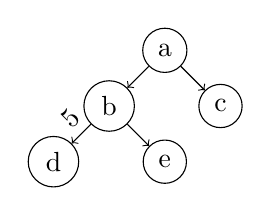
\begin{tikzpicture}[main/.style = {draw, circle}] 
\node[main] (a) {a}; 
\node[main] (b) [below left of=a] {b}; 
\node[main] (c) [below right of=a] {c}; 
\node[main] (d) [below left of=b] {d}; 
\node[main] (e) [below right of=b] {e}; 
\draw[->] (a) -- (b);
\draw[->] (a) -- (c);
\draw[->] (b) -- node[midway, above right, sloped, pos=1] {5} (d) ;
\draw[->] (b) -- (e);
\end{tikzpicture}

\subsubsection{Parsen}
Die Datei liegen in einer Datei mit der Endung \textit{*.grph} vor. Die Syntax des Graphs ist durch eine EBNF spezifiziert:
\begin{verbatim}
("#directed:",name) | ("#undirected:",name) ;
node1[":"attr1],[{" "}"-"{" "}node2,[":"attr2],[" "{" "}"("edge")"],["::"weight]],{" "}";";
\end{verbatim}
Die begrenzte Eignung einer EBNF für das Parsen der Datei in Java führte zur Entscheidung, diese durch einen regulären Ausdruck (Regex) zu ersetzen. Java bietet dabei eine effiziente Funktionalität zur Extraktion von Daten mittels Regex.
\newline \newline
Durch den Einsatz von Regex kann die Datei zeilenweise analysiert werden. Hierbei wird die erste Zeile gesondert behandelt, da sie die Informationen des Graphen enthält (nachfolgend als "Header" bezeichnet). Die übrigen Zeichen repräsentieren die Kanten und Knoten des Graphen (nachfolgend als "Body" bezeichnet). Die Informationen des zugrundeliegenden Graphen werden in einem "DTO GrphStructure" gespeichert, während die Details zu den einzelnen Zeilen des Bodys im "DTO GrphLine" festgehalten werden. Der DTO lässt sich anschließend in ein Graph-Objekt von Graphstream konvertieren. Kanten ohne Gewichtung erhalten automatisch eine Gewichtung von \textit{1}.

\subsubsection{Speichern}
Bei der Speicherung eines Graphen wird der zugrundeliegende Graph in ein "DTO GrphStructure" konvertiert, welches anschließend durch einen Writer in eine Datei gespeichert werden kann. Unabhängig ob es sich beim übergebenen Writer um einen StringWriter oder einen FileWriter handelt - die konkrete Implementierung ist dabei irrelevant. Diese Herangehensweise verbessert maßgeblich die Testbarkeit, da keine Abhängigkeiten zum Dateisystem besteht.

\subsection{Visualisierung}
Die Visualisierung wird von der Graphstream Library übernommen, wobei lediglich mithilfe von CSS Feinabstimmungen vorgenommen werden.

\clearpage
\subsection{Klassen}
\begin{figure}[h!]
    \centering
    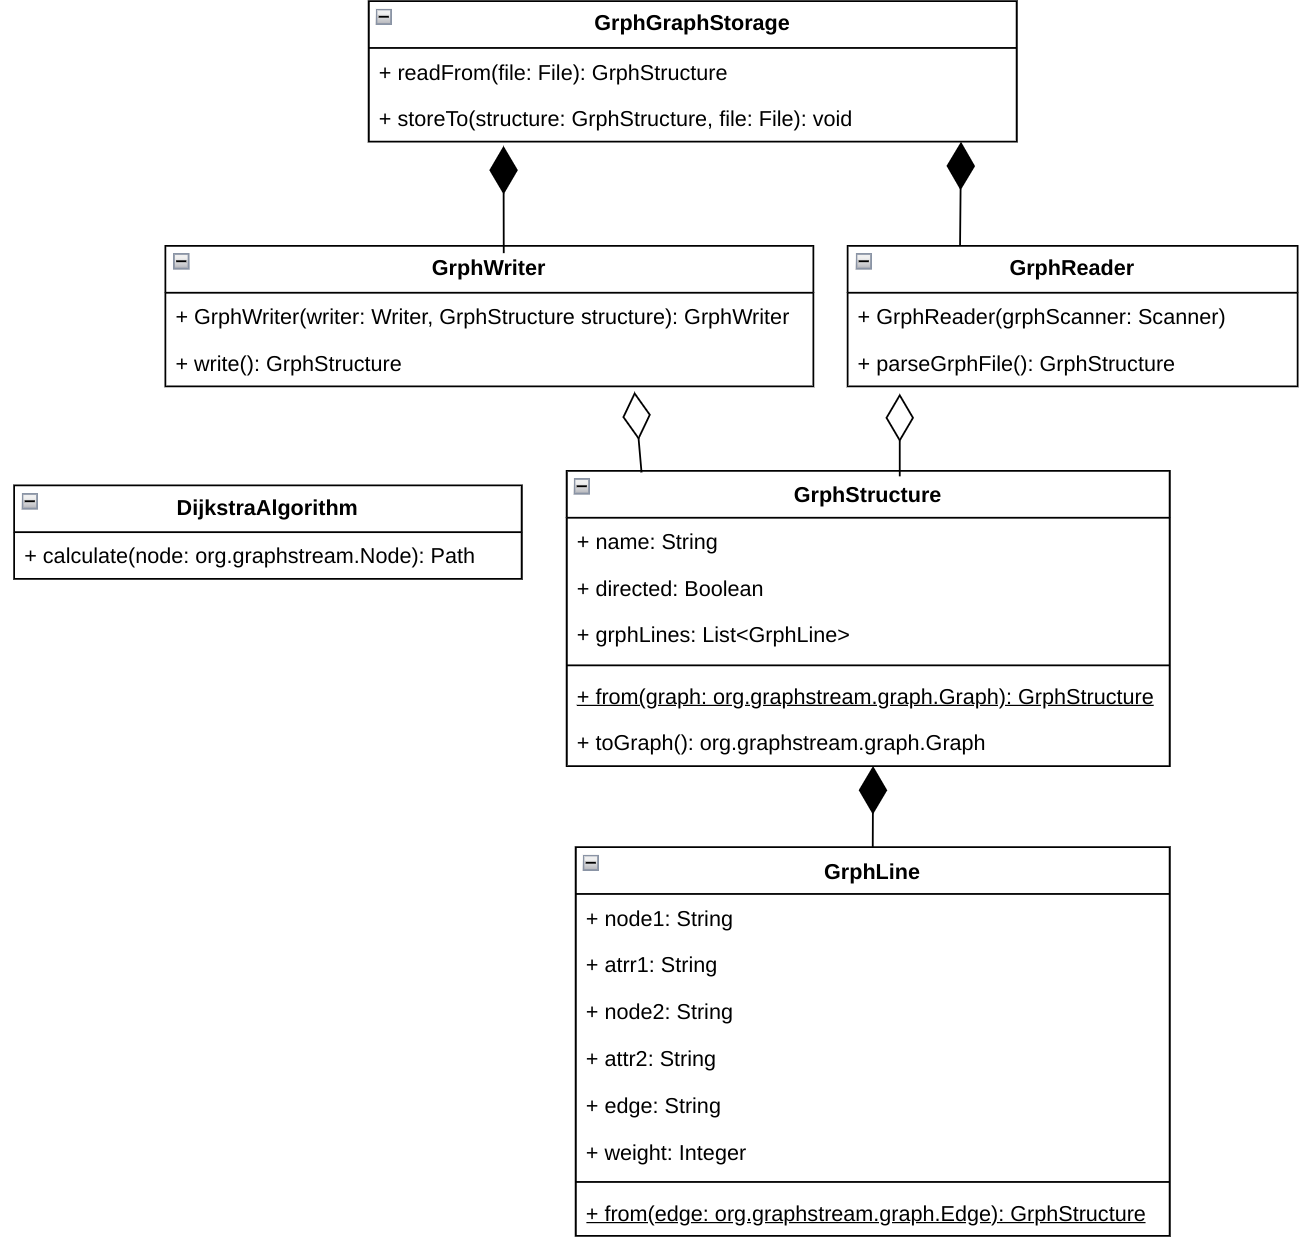
\includegraphics[scale=0.20]{Figs/Klassendiagramm.png}
    \caption{UML Klassendiagramm}
    \label{fig:enter-label}
\end{figure}

\subsubsection{GrphGraphStorage}
Diese Klasse ist verantwortlich für das Speichern und Lesen von Dateien. Sie wird vom Benutzerinterface aufgerufen, um eine vorgegebene Datei zu laden oder zu speichern. Im Falle des Lesens erzeugt sie einen Scanner für die zu lesende Datei. Beim Schreiben wird der entsprechende Writer definiert.

\subsubsection{GrphReader}
Die Klasse erwartet einen Scanner, der auf eine *.grph-Datei zeigt. Sie liest die Datei zeilenweise ein und gibt eine GrphStructure zurück, die die Daten des Graphen enthält. Hierbei wird ein regulärer Ausdruck verwendet, um die Daten zu extrahieren.

\subsubsection{GrphWriter}
Die Klasse erwartet einen Writer sowie eine GrphStructure als Eingabe. Sie umfasst Funktionalitäten zum Erstellen eines gültigen Header in der Syntax einer *.grph-Datei aus einer gegebenen GraphStructure. Des Weiteren schreibt sie jede GraphLine auch in den übergebenen Writer.

\subsubsection{GrphStructure}
Beinhaltet eine 1:1-Abbildung der Grph-Datei und enthält Informationen wie Name, Typ des Graphs (gerichtet/ungerichtet) sowie eine Referenz zu den zugehörigen Zeilen der Knoten-Kanten-Beziehung. Die Klasse umfasst eine Methode, die die GrphStructure in einen Graphen umwandelt, sowie einen Rückweg (zum Beispiel für das Speichern des Graphen), der ebenfalls über eine Methode realisiert wird.

\subsubsection{GrphLine}
Enthält die Informationen zu einer Zeile im Body der Grph-Datei. Speichert sämtliche zugehörigen Informationen wie Attribute, Kantennamen und Gewichtung.

\subsubsection{DijkstraAlgorithm}
Die Implementierung basiert auf dem von Dijkstra entworfenen Algorithmus und verwendet dabei ein Graph-Objekt von Graphstream zur Berechnung. Ausgehend von einem gegebenen Startknoten werden alle Routen zu erreichbaren Knoten berechnet. Die Vorgänger und die Distanz zum Startknoten werden dabei als Attribute am GraphStream-Objekt gespeichert.

\subsection{Algorithmus}
Bei dem implementierten Algorithmus handelt es sich um einen Dijkstra-Algorithmus. Die berechneten Vorgänger und die Distanzen werden als Attribute am Graph-Objekt gespeichert. Die zu untersuchenden Knoten werden in einem Priority Heap gespeichert, in Java durch die Klasse PriorityQueue.

Die konkrete Implementierung orientiert sich am folgenden Pseudocode:
\begin{lstlisting}[caption={Pseudocode Dijkstra von Wikipedia \cite{pseudocode}},captionpos=b]
function Dijkstra(Graph, source):
	for each vertex v in Graph.Vertices:
                dist[v] <- INFINITY
                prev[v] <- UNDEFINED
                add v to Q
	dist[source] <- 0

	while Q is not empty:
		u <- vertex in Q with min dist[u]
        	remove u from Q
        
		for each neighbor v of u still in Q:
			alt <- dist[u] + Graph.Edges(u, v)
			if alt < dist[v]:
				dist[v] <- alt
				prev[v] <- u
	return dist[], prev[]
\end{lstlisting}